\chapter{Immunité innée et inflammation}\label{ch:b3:innate-immunity}

Une écharde sous la peau y introduit dix mille bactéries qui vont
doubler toutes les demi-heures. En quelques minutes les vaisseaux
alentour se dilatent et laissent fuir le plasma~; en une heure les
premiers \omterm{def:b3:innate-immunity:innate}{neutrophiles} se sont extraits du sang et rampent vers les
intrus le long d'une piste chimique~; en un jour le site est rouge,
chaud, gonflé et douloureux --- les quatre signes de l'\omterm{def:b3:innate-immunity:inflammation}{inflammation} que
Celse a énumérés il y a deux mille ans --- et les bactéries sont mortes,
dévorées vivantes par des cellules qui les ont reconnues comme
étrangères sans les avoir jamais rencontrées. C'est l'\omterm{def:b3:innate-immunity:innate}{immunité innée}~:
la défense que possède tout animal, prête avant l'infection, inscrite
dans le génome plutôt qu'apprise. Elle est rapide, c'est elle qui tue la
plupart des envahisseurs, et c'est elle qui avertit l'immunité apprise,
plus lente, du chapitre suivant qu'il y a quelque chose à apprendre. Ses
excès --- choc septique, \omterm{def:b3:innate-immunity:inflammation}{inflammation} chronique, fièvres des maladies
auto-inflammatoires --- sont aussi instructifs que ses réussites.

\section{Les couches et les cellules}

\begin{definition}[L'immunité innée]\label{def:b3:innate-immunity:innate}
\index{immunité innée}\index{neutrophile}\index{macrophage}\index{cellule dendritique}\index{cellule tueuse naturelle}\index{barrière}
L'\emph{immunité innée} est l'ensemble des défenses présentes avant
toute exposition, codées par des gènes germinaux qui ne se réarrangent
pas, reconnaissant des caractères conservés des microbes plutôt que des
individus précis, agissant en quelques minutes à quelques heures et
(sous réserve) sans mémoire. Sa première couche est celle des
\emph{barrières}~: la kératine de la peau, le mucus et les cils des
voies aériennes, l'acidité de l'estomac, le lavage de l'urine et des
larmes, le lysozyme qui coupe le \omterm{def:b3:bacteriology:envelope}{peptidoglycane}, les \emph{peptides
antimicrobiens} (défensines, cathélicidines) qui perforent les membranes
microbiennes, et le \omterm{def:b3:microbiomes:symbiosis}{microbiote} commensal qui occupe les niches
(\cref{ch:b3:microbiomes}). Ses cellules, toutes de la lignée myéloïde
sauf la dernière~: les \emph{neutrophiles}, \qty{60}{\%} des leucocytes
du sang, $10^{11}$ produits par jour, vivant un jour, les premiers
arrivés et les principaux tueurs de bactéries~; les \emph{macrophages},
résidents de longue vie de tous les tissus (cellules de Kupffer dans le
foie, microglie dans le cerveau, macrophages alvéolaires dans le poumon)
qui mangent, nettoient et donnent l'alerte~; les \emph{cellules
dendritiques}, qui échantillonnent les tissus et portent leur récolte
aux ganglions lymphatiques~; les mastocytes, les basophiles et les
éosinophiles, armés contre les parasites et responsables de l'allergie~;
et les \emph{cellules tueuses naturelles} (NK), lymphocytes qui tuent à
vue les cellules infectées ou transformées.
\end{definition}

\begin{proof}[Faits expérimentaux]
Metchnikoff (1882), à Messine, enfonça une épine de rose dans une larve
transparente d'étoile de mer et vit, le lendemain matin, des cellules
mobiles se presser autour~; il avait vu les mêmes cellules engloutir des
particules alimentaires et des grains de colorant, et proposa qu'elles
engloutissaient aussi les microbes --- les \emph{phagocytes}, agents
d'une défense de l'hôte qu'il traqua ensuite chez tous les animaux qu'il
put trouver, de l'amibe à l'homme. Il partagea le prix Nobel de 1908
avec Ehrlich, dont les anticorps représentaient la vue humorale
opposée~; tous deux avaient raison, et un siècle plus tard les deux
moitiés de l'immunité se révélèrent un seul système, la moitié innée
instruisant l'adaptative.
\end{proof}

\begin{omfigure}
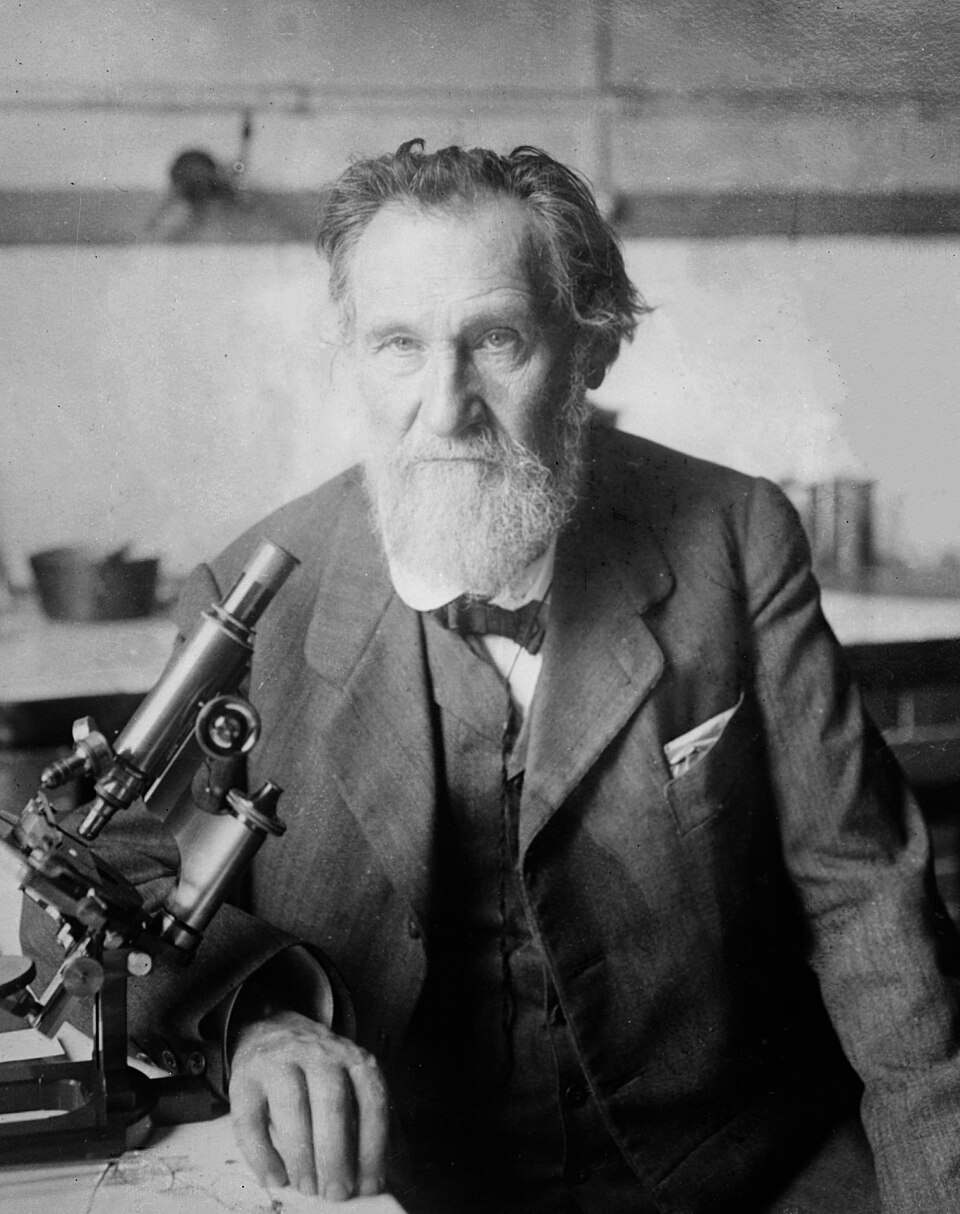
\includegraphics[width=0.30\linewidth]{images/book5/metchnikoff.jpg}\hspace{0.04\linewidth}
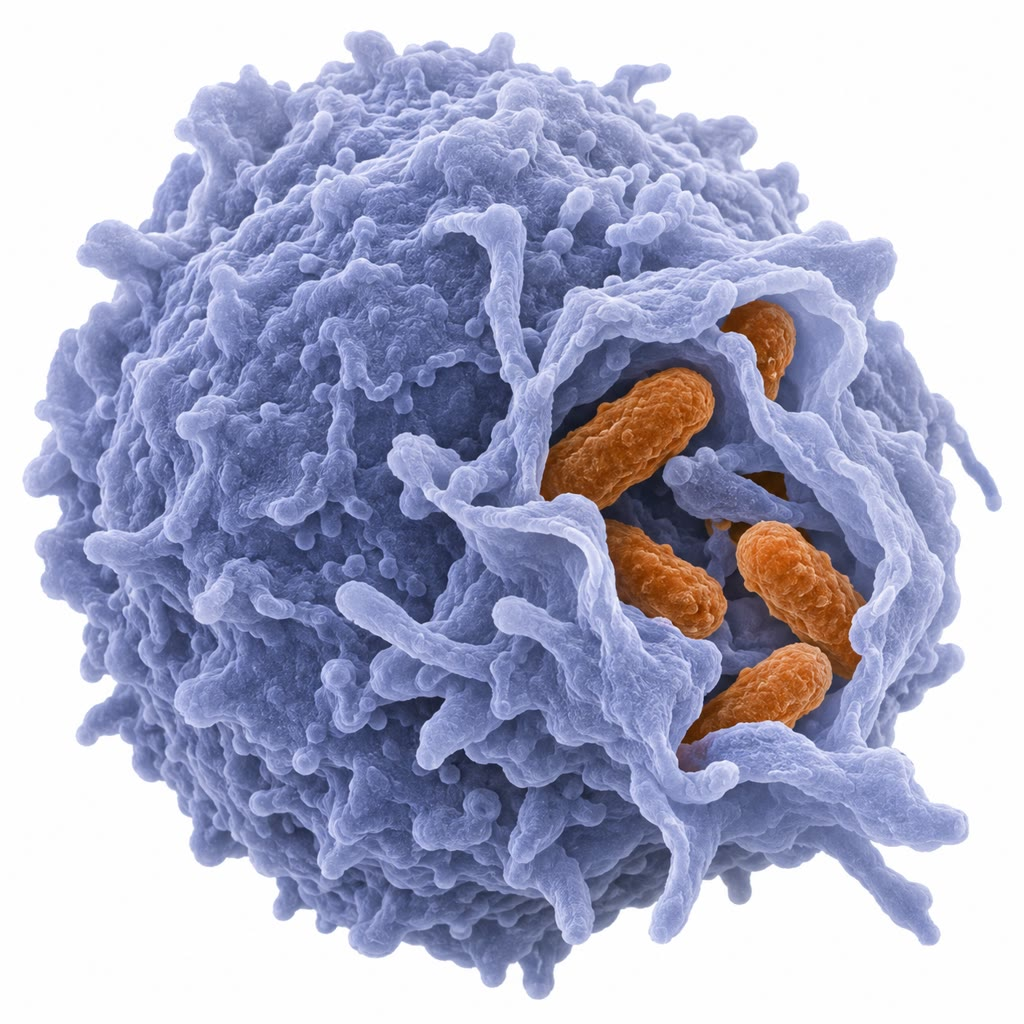
\includegraphics[width=0.30\linewidth]{images/book5/ai/b5-15-neutrophil-phagocytosis.jpg}\hspace{0.04\linewidth}
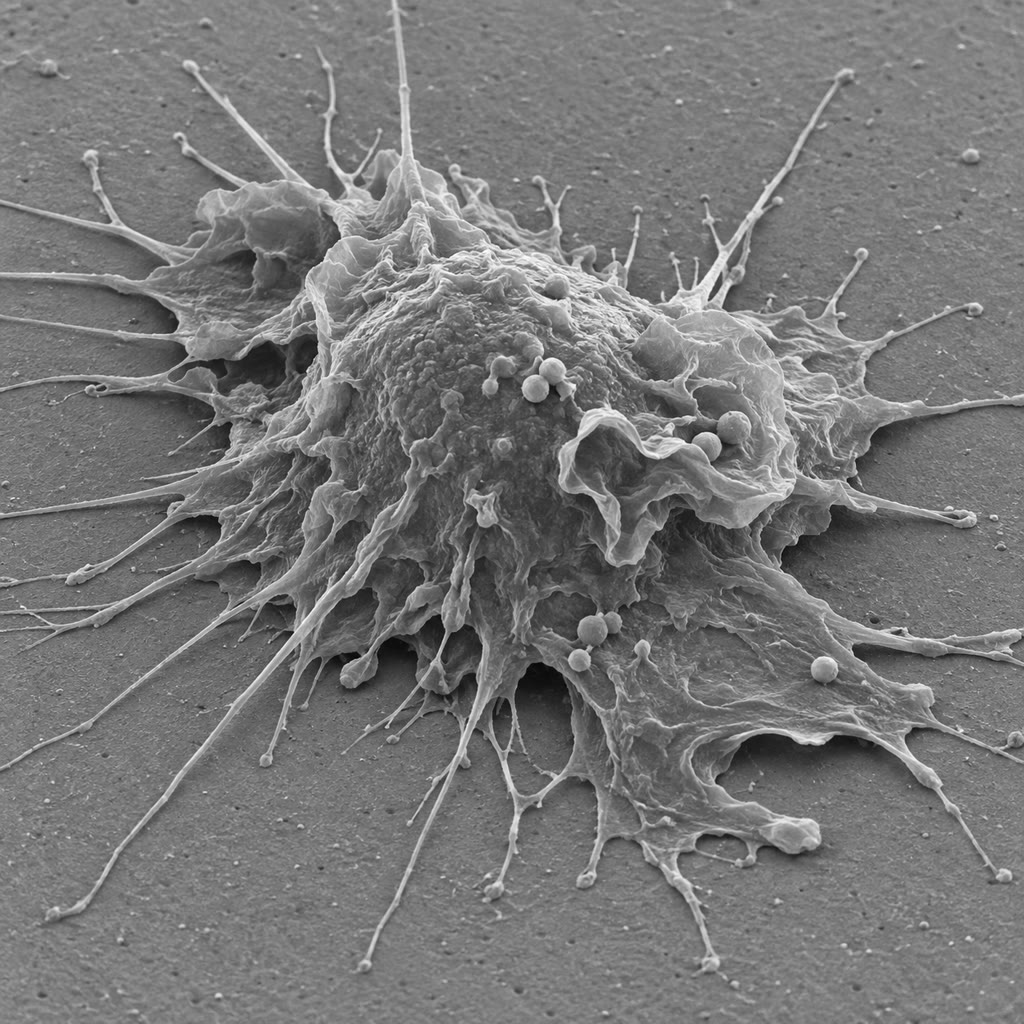
\includegraphics[width=0.30\linewidth]{images/book5/ai/b5-15-macrophage.jpg}

{\small Élie Metchnikoff, qui vit des phagocytes se rassembler autour
d'une épine dans une larve d'étoile de mer et fonda l'immunologie
cellulaire (Library of Congress, domaine public). Au centre~: un
\omterm{def:b3:innate-immunity:innate}{neutrophile} engloutissant des bactéries. À droite~: un \omterm{def:b3:innate-immunity:innate}{macrophage}
étalant ses membranes en collerette sur une surface.}
\end{omfigure}

\section{Reconnaître l'ennemi}

\begin{definition}[La reconnaissance de motifs]\label{def:b3:innate-immunity:prr}
\index{récepteur de reconnaissance de motifs}\index{motif moléculaire associé aux pathogènes}\index{récepteur de type Toll}\index{motif moléculaire associé aux dégâts}\index{inflammasome}
Les cellules innées reconnaissent des \emph{motifs moléculaires associés
aux pathogènes} (PAMP)~: des molécules communes à des classes entières
de microbes, essentielles à ceux-ci et absentes de l'hôte --- le
\omterm{def:b3:bacteriology:envelope}{lipopolysaccharide} des parois à \omterm{def:b3:bacteriology:envelope}{Gram négatif}, le \omterm{def:b3:bacteriology:envelope}{peptidoglycane} et
l'acide lipotéichoïque des \omterm{def:b3:bacteriology:envelope}{Gram positif}, la flagelline, les
$\beta$-glucanes fongiques, l'ARN double brin, l'ARN sans coiffe en
5$'$, l'ADN à \omterm{def:b3:chromatin-epigenetics:methylation}{CpG} non méthylés, l'ADN dans le cytosol. Les récepteurs
sont les \emph{récepteurs de reconnaissance de motifs} (PRR), quelques
dizaines en tout, chacun codé par un gène~: les \emph{récepteurs de type
Toll} (TLR) de la surface et des \omterm{def:b3:membrane-traffic:endocytosis}{endosomes} (TLR4 pour le
\omterm{def:b3:bacteriology:envelope}{lipopolysaccharide}, TLR5 pour la flagelline, TLR3 pour l'ARN double
brin, TLR9 pour l'ADN \omterm{def:b3:chromatin-epigenetics:methylation}{CpG})~; les protéines cytosoliques NOD pour les
fragments de \omterm{def:b3:bacteriology:envelope}{peptidoglycane}, RIG-I pour l'ARN viral, cGAS--STING pour
l'ADN cytosolique~; les lectines de type C pour les sucres fongiques.
Les mêmes récepteurs, ou d'autres des mêmes familles, reconnaissent les
\emph{motifs moléculaires associés aux dégâts} (DAMP) libérés par les
cellules lésées --- ATP, acide urique, la protéine nucléaire HMGB1,
l'ADN mitochondrial --- de sorte qu'une lésion stérile enflamme elle
aussi. La liaison active les facteurs de transcription NF-$\kappa$B et
les facteurs régulateurs de l'interféron, qui allument \omterm{def:b3:innate-immunity:inflammation}{cytokines},
\omterm{def:b3:innate-immunity:inflammation}{chimiokines}, molécules d'adhérence et gènes antimicrobiens en moins
d'une heure~; une partie des capteurs cytosoliques assemblent
l'\emph{inflammasome}, une plate-forme qui active la caspase-1 pour
couper l'interleukine-1$\beta$ en sa forme active et pour déclencher la
mort inflammatoire appelée \omterm{def:b3:cell-cycle-apoptosis:other}{pyroptose} (\cref{ch:b3:cell-cycle-apoptosis}).
\end{definition}

\begin{proof}[Faits expérimentaux]
Janeway proposa en 1989 que le système immunitaire adaptatif ne répond
pas à l'antigène seul mais a besoin d'un signal venu de récepteurs innés
ayant reconnu des motifs microbiens --- l'explication de la nécessité
d'adjuvants dans les vaccins, «~le sale petit secret de
l'immunologiste~». Hoffmann (1996) découvrit que \emph{Drosophila},
privée du récepteur Toll connu pour son rôle dans la mise en place du
plan embryonnaire, ne pouvait monter de réponse antifongique et mourait
couverte de moisissure~; Beutler (1998) rapporta la résistance au
\omterm{def:b3:bacteriology:envelope}{lipopolysaccharide} d'une souche de souris, qui survivait à des doses
d'endotoxine mortelles pour les autres et n'éliminait pas les infections
à \omterm{def:b3:bacteriology:envelope}{Gram négatif}, à une mutation de l'homologue mammifère TLR4. Le
récepteur de l'endotoxine, cherché pendant cinquante ans, était un Toll.
\end{proof}

\begin{omfigure}
\begin{tikzpicture}[every node/.style={font=\scriptsize}, >=stealth]
  % membrane
  \draw[very thick, omDef] (0,3.0) -- (11.5,3.0); \draw[very thick, omDef] (0,2.7) -- (11.5,2.7);
  \node[above] at (0.5,3.05) {extérieur}; \node[below] at (0.5,2.65) {cytosol};
  % TLR4 with LPS
  \draw[thick, fill=omProp!35] (2.2,2.4) rectangle (2.6,3.9); \draw[thick, fill=omProp!35] (2.9,2.4) rectangle (3.3,3.9);
  \fill[omThm] (2.75,4.1) circle (0.14); \node[above] at (2.75,4.25) {LPS (un PAMP)};
  \node[right, align=left] at (3.4,3.5) {dimère de TLR4\\avec MD2};
  % signalling
  \node[draw, thick, rounded corners, fill=omDef!20] (myd) at (2.75,1.7) {MyD88 et kinases};
  \node[draw, thick, rounded corners, fill=omDef!20] (nfkb) at (2.75,0.6) {NF-$\kappa$B libéré};
  \node[draw, thick, rounded corners, fill=omMeth!25, align=center] (genes) at (2.75,-0.8) {TNF, IL-1$\beta$, IL-6, IL-8~;\\molécules d'adhérence~; iNOS};
  \draw[->, thick] (2.75,2.4) -- (myd); \draw[->, thick] (myd) -- (nfkb); \draw[->, thick] (nfkb) -- (genes);
  \node[right, font=\tiny] at (3.3,1.2) {en moins d'une heure};
  % cytosolic sensors
  \node[draw, thick, rounded corners, fill=omProp!25, align=center] (rig) at (6.9,1.9) {RIG-I~: ARN viral\\cGAS--STING~: ADN cytosolique};
  \node[draw, thick, rounded corners, fill=omMeth!25] (ifn) at (6.9,-0.2) {interféron de type~I};
  \draw[->, thick] (rig) -- node[midway, right] {IRF3, IRF7} (ifn);
  \node[draw, thick, rounded corners, fill=omThm!20, align=center] (nlrp) at (10.9,1.9) {inflammasome NLRP3~:\\cristaux, ATP, pores};
  \node[draw, thick, rounded corners, fill=omMeth!25, align=center] (il1) at (10.9,-0.8) {caspase-1~: IL-1$\beta$\\libérée~; pyroptose};
  \draw[->, thick] (nlrp) -- (il1);
  \draw[->, thick, dashed] (genes.south) -- ++(0,-0.5) -| (il1.south) node[pos=0.25, below, font=\tiny] {pro-IL-1$\beta$ fournie par la voie TLR};
\end{tikzpicture}

{\small Trois bras de la reconnaissance de motifs. Un \omterm{def:b3:innate-immunity:prr}{récepteur de type
Toll} de surface lié par le \omterm{def:b3:bacteriology:envelope}{lipopolysaccharide} signale par NF-$\kappa$B
vers les \omterm{def:b3:innate-immunity:inflammation}{cytokines} inflammatoires~; les capteurs cytosoliques d'acide
nucléique viral induisent l'interféron~; l'\omterm{def:b3:innate-immunity:prr}{inflammasome} transforme le
précurseur stocké de l'interleukine-1 en \omterm{def:b3:innate-immunity:inflammation}{cytokine} active.}
\end{omfigure}

\begin{definition}[Le complément]\label{def:b3:innate-immunity:complement}
\index{complément}\index{convertase C3}\index{opsonisation}\index{complexe d'attaque membranaire}\index{anaphylatoxine}
Le \emph{complément} est un système d'une trentaine de protéines
plasmatiques, \qty{10}{\%} des globulines du sérum, qui marque et
détruit les microbes par une cascade d'activations protéolytiques. Trois
voies convergent vers le clivage de la protéine centrale C3~: la voie
\emph{classique}, déclenchée par C1q liant des anticorps sur une surface
(ou la \omterm{prop:b3:innate-immunity:systemic}{protéine C réactive}, ou des cellules apoptotiques)~; la voie
\emph{des lectines}, déclenchée par la lectine liant le mannose qui
reconnaît les sucres microbiens~; et la voie \emph{alterne}, où C3
s'hydrolyse spontanément à faible taux et où le C3b ainsi formé se fixe
sur toute surface rencontrée. Chaque voie construit une \emph{convertase
C3}, enzyme qui clive d'autres C3~; le C3b qu'elle dépose par covalence
sur la surface construit à son tour davantage de convertase --- une
boucle d'amplification --- si bien qu'une bactérie se couvre de millions
de C3b en quelques minutes. Le C3b est une \emph{opsonine}~: les
phagocytes en portent les récepteurs et mangent ce qu'il recouvre. Les
petits fragments C3a et C5a sont des \emph{anaphylatoxines} qui dilatent
les vaisseaux, attirent les \omterm{def:b3:innate-immunity:innate}{neutrophiles} et activent les mastocytes. Et
C5b assemble C6--C9 en un \emph{complexe d'attaque membranaire}, un pore
de \qty{10}{nm} qui lyse les bactéries à \omterm{def:b3:bacteriology:envelope}{Gram négatif} et les \omterm{def:b3:virology:virus}{virus}
enveloppés. Les cellules de l'hôte sont épargnées parce qu'elles portent
des régulateurs --- facteur H, CD55, CD59 --- qui démontent la
convertase et bloquent le pore sur leurs propres surfaces~; les
microbes, qui en sont dépourvus, sont consumés par la boucle.
\end{definition}

\begin{theorem}[La boucle du complément comme discriminateur cinétique]\label{thm:b3:innate-immunity:complement}
\index{complément!boucle d'amplification}
Soit $B(t)$ le nombre de molécules de C3b déposées sur une surface. Le
C3b est déposé à un faible taux constant $k_{0}$ par le bruit de fond du
C3, et chaque C3b déposé construit de la convertase qui en dépose
davantage au taux $a$ par C3b et par seconde, tandis que les régulateurs
(hôte) et la décroissance retirent de l'activité convertase au taux $d$
par C3b et par seconde~:
\[
\frac{\mathrm{d}B}{\mathrm{d}t} = k_{0} + (a - d)\,B .
\]
Sur une surface où $a > d$ --- un microbe, sans régulateurs ---
$B(t) = \bigl[k_{0}/(a-d)\bigr]\bigl(e^{(a-d)t} - 1\bigr)$ croît
exponentiellement avec la constante de temps $1/(a - d)$~; sur une
surface de l'hôte où $d > a$, $B$ tend vers la faible valeur
stationnaire $k_{0}/(d - a)$. Les mêmes molécules, aux mêmes
concentrations, déposent un million de C3b sur une bactérie en quelques
minutes et quelques dizaines sur la cellule voisine~: la distinction
entre le soi et le non-soi n'est pas faite par une reconnaissance mais
par le signe de $a - d$.
\end{theorem}
\begin{proof}
L'équation est linéaire à coefficients constants. Pour $a \ne d$ le
point fixe est $B^{*} = -k_{0}/(a-d)$~; en posant $B = B^{*} + u$,
$\mathrm{d}u/\mathrm{d}t = (a-d)u$, donc $u = u_{0}e^{(a-d)t}$ et avec
$B(0) = 0$, $B(t) = \bigl[k_{0}/(a-d)\bigr](e^{(a-d)t} - 1)$. Pour $a > d$
cela croît sans borne (jusqu'à épuisement du C3 ou de la surface)~; pour
$a < d$ l'exponentielle décroît et $B \to k_{0}/(d-a) > 0$. Avec
$k_{0} = 1$ par seconde et $a - d = \qty{0.1}{s^{-1}}$ sur une bactérie,
$B(\qty{2}{min})
= 10(e^{12} - 1) \approx 1.6\times 10^{6}$~; avec $d - a =
\qty{0.1}{s^{-1}}$ sur une cellule de l'hôte, $B^{*} = 10$.
\end{proof}

\begin{omfigure}
\begin{tikzpicture}
\begin{axis}[
  width=0.66\linewidth, height=5.6cm,
  axis x line=bottom, axis y line=left,
  xmin=0, xmax=150, ymin=1, ymax=1e7, ymode=log,
  xlabel={secondes}, ylabel={C3b déposé},
  xlabel style={font=\small, at={(axis description cs:0.5,-0.12)}, anchor=north}, ylabel style={font=\small},
  tick label style={font=\small}, xtick={0,30,60,90,120,150},
  clip=false,
]
\addplot[very thick, omThm, domain=1:150, samples=80] {10*(exp(0.1*x)-1)};
\addplot[very thick, omDef, domain=1:150, samples=80] {10*(1-exp(-0.1*x))};
\node[font=\scriptsize, omThm, anchor=east] at (axis cs:100,2e5) {microbe~: $a > d$, exponentiel};
\node[font=\scriptsize, omDef, anchor=south west] at (axis cs:60,14) {cellule de l'hôte~: $d > a$, sature à $k_{0}/(d-a)$};
\end{axis}
\end{tikzpicture}

{\small La boucle du \omterm{def:b3:innate-immunity:complement}{complément} sur deux surfaces avec $k_{0} = 1$ par
seconde et $|a - d| = \qty{0.1}{s^{-1}}$~: sur un microbe dépourvu de
régulateurs le C3b croît exponentiellement et atteint le million en deux
minutes~; sur une cellule de l'hôte munie de régulateurs il plafonne à
dix.}
\end{omfigure}

\begin{omfigure}
\begin{tikzpicture}[every node/.style={font=\scriptsize}, >=stealth]
  \node[draw, thick, rounded corners, fill=omDef!20, align=center] (cl) at (-4.2,3.0) {voie classique~:\\C1q sur un anticorps\\ou la protéine C réactive};
  \node[draw, thick, rounded corners, fill=omDef!20, align=center] (le) at (0,3.0) {voie des lectines~:\\lectine liant le mannose\\sur les sucres microbiens};
  \node[draw, thick, rounded corners, fill=omDef!20, align=center] (al) at (4.2,3.0) {voie alterne~:\\bruit de fond du C3,\\C3b sur toute surface};
  \node[draw, thick, rounded corners, fill=omProp!35, minimum width=3cm] (conv) at (0,1.2) {convertase C3};
  \node[draw, thick, rounded corners, fill=omThm!25, align=center] (c3b) at (0,-0.4) {C3 $\to$ C3b (sur la surface) $+$ C3a};
  \draw[->, thick] (cl) -- (conv); \draw[->, thick] (le) -- (conv); \draw[->, thick] (al) -- (conv);
  \draw[->, thick] (conv) -- (c3b);
  \draw[->, very thick, omThm] (c3b.east) .. controls (3.2,-0.4) and (3.2,1.2) .. (conv.east) node[pos=0.5, right, align=left] {boucle d'amplification~:\\le C3b fait plus de convertase};
  \node[draw, thick, rounded corners, fill=omMeth!25, align=center] (ops) at (-4.4,-2.2) {opsonisation~:\\les phagocytes mangent\\ce que le C3b couvre};
  \node[draw, thick, rounded corners, fill=omMeth!25, align=center] (ana) at (0,-2.2) {C3a, C5a~:\\les vaisseaux se dilatent,\\neutrophiles et mastocytes recrutés};
  \node[draw, thick, rounded corners, fill=omMeth!25, align=center] (mac) at (4.4,-2.2) {C5b--C9~:\\complexe d'attaque\\membranaire, lyse};
  \draw[->, thick] (c3b) -- (ops); \draw[->, thick] (c3b) -- (ana); \draw[->, thick] (c3b) -- (mac);
  \node[draw, thick, rounded corners, fill=gray!15, align=center] (reg) at (-4.4,1.2) {régulateurs de l'hôte~:\\facteur H, CD55, CD59};
  \draw[-|, thick, gray!60!black] (reg) -- (conv);
\end{tikzpicture}

{\small Le \omterm{def:b3:innate-immunity:complement}{complément}. Trois routes construisent une \omterm{def:b3:innate-immunity:complement}{convertase C3}~; le
C3b qu'elle dépose en construit davantage (la boucle du théorème), et le
C3b déposé opsonise, les fragments enflamment et le complexe terminal
lyse. Les cellules de l'hôte portent des régulateurs qui coupent la
boucle (et, avec CD59, bloquent le pore) sur leurs propres membranes.}
\end{omfigure}

\section{L'inflammation}

\begin{definition}[L'inflammation aiguë]\label{def:b3:innate-immunity:inflammation}
\index{inflammation}\index{cytokine}\index{chimiokine}\index{extravasation}\index{sélectine}\index{intégrine}
L'\emph{inflammation} est la réponse d'un tissu vascularisé à une lésion
ou à une infection, orchestrée par les \emph{cytokines} --- les petites
protéines de signalisation des cellules immunitaires, ici surtout le
TNF, l'interleukine-1 et l'interleukine-6 des \omterm{def:b3:innate-immunity:innate}{macrophages} activés --- et
par les \emph{chimiokines}, les cytokines qui dirigent la migration. Ses
étapes expliquent les signes de Celse. L'histamine des mastocytes, le
monoxyde d'azote et les prostaglandines dilatent les artérioles~:
\emph{rougeur} et \emph{chaleur}. L'endothélium des veinules se contracte
et laisse fuir le plasma, dont les protéines --- \omterm{def:b3:innate-immunity:complement}{complément}, anticorps,
facteurs de la coagulation --- inondent le tissu~: \emph{gonflement}. La
bradykinine et la prostaglandine E$_{2}$ sensibilisent les terminaisons
nerveuses~: \emph{douleur}. Et les leucocytes arrivent par
\emph{extravasation}~: le TNF et l'interleukine-1 font exposer à
l'endothélium des \emph{sélectines}, sur lesquelles les \omterm{def:b3:innate-immunity:innate}{neutrophiles} de
passage s'accrochent et roulent~; les chimiokines (interleukine-8) de la
surface endothéliale activent les \emph{intégrines} des \omterm{def:b3:innate-immunity:innate}{neutrophiles},
qui se lient fermement aux molécules d'adhérence endothéliales et
arrêtent la cellule~; et le \omterm{def:b3:innate-immunity:innate}{neutrophile} se faufile entre les cellules
endothéliales et suit le gradient de chimiokine dans le tissu --- toute
la séquence en quelques minutes, à raison d'un million de cellules par
heure vers un site infecté.
\end{definition}

\begin{omfigure}
\begin{tikzpicture}[every node/.style={font=\scriptsize}, >=stealth]
  % vessel wall
  \fill[omThm!10] (0,0) rectangle (12,2.3); \node[left, omThm!70!black, anchor=north east] at (12,2.25) {sang, qui coule $\rightarrow$};
  \foreach \x in {0,1.5,3,4.5,6,7.5,9,10.5} \draw[thick, fill=omDef!30] (\x,-0.05) rectangle (\x+1.45,0.35);
  \node[right] at (0.1,-0.35) {endothélium};
  \fill[omMeth!8] (0,-1.7) rectangle (12,-0.45); \node[right, omMeth!60!black] at (0.1,-1.55) {tissu};
  % bacteria and chemokine gradient
  \foreach \p in {(10.6,-1.1),(11.0,-0.9),(11.3,-1.2)} \fill[omProp] \p ellipse (0.14 and 0.07);
  \node[below, omProp] at (11.0,-1.35) {bactéries};
  \node[below, font=\tiny] at (8.0,-0.5) {gradient de chimiokine $\rightarrow$};
  % neutrophils in sequence
  \draw[thick, fill=white] (1.2,1.1) circle (0.3); \node[above] at (1.2,1.45) {1. circulation};
  \draw[thick, fill=white] (3.4,0.68) circle (0.3); \node[above] at (3.4,1.05) {2. roulement sur les sélectines};
  \draw[omThm, thick] (3.1,0.45) -- (3.05,0.35); \draw[omThm, thick] (3.4,0.38) -- (3.4,0.35); \draw[omThm, thick] (3.7,0.45) -- (3.75,0.35);
  \draw[thick, fill=white] (6.0,0.62) ellipse (0.38 and 0.26); \node[above, align=center] at (6.0,0.95) {3. adhérence ferme\\(intégrines)};
  \draw[thick, fill=white] (8.25,0.18) ellipse (0.2 and 0.42); \node[above, align=center] at (8.4,0.95) {4. passage\\entre les cellules};
  \draw[thick, fill=white] (9.6,-1.0) circle (0.3); \node[left] at (9.25,-1.0) {5. reptation vers le site};
  \draw[->, thick, gray] (1.5,1.05) -- (3.0,0.8); \draw[->, thick, gray] (3.7,0.68) -- (5.6,0.62); \draw[->, thick, gray] (6.4,0.5) -- (8.0,0.4); \draw[->, thick, gray] (8.3,-0.3) -- (9.3,-0.8);
  % TNF label
  \node[below, align=center, font=\tiny] at (4.0,-1.75) {le TNF et l'IL-1 des macrophages du tissu font exposer à l'endothélium\\les sélectines et les molécules d'adhérence qui retiennent les neutrophiles};
\end{tikzpicture}

{\small L'\omterm{def:b3:innate-immunity:inflammation}{extravasation}. Les \omterm{def:b3:innate-immunity:inflammation}{cytokines} des \omterm{def:b3:innate-immunity:innate}{macrophages} du tissu rendent
la paroi de la veinule collante~; un \omterm{def:b3:innate-immunity:innate}{neutrophile} de passage s'accroche
aux \omterm{def:b3:innate-immunity:inflammation}{sélectines} et roule, est arrêté par ses \omterm{def:b3:innate-immunity:inflammation}{intégrines}, se faufile entre
les cellules endothéliales et suit le gradient de \omterm{def:b3:innate-immunity:inflammation}{chimiokine} jusqu'aux
bactéries.}
\end{omfigure}

\begin{proposition}[La fièvre, la phase aiguë et la résolution]\label{prop:b3:innate-immunity:systemic}
\index{fièvre}\index{réponse de phase aiguë}\index{protéine C réactive}\index{résolution de l'inflammation}
L'interleukine-1, le TNF et l'interleukine-6 agissent aussi à distance.
Dans l'hypothalamus ils induisent la prostaglandine E$_{2}$, qui élève
la consigne de la température corporelle~: la \emph{fièvre}, qui
ralentit bien des bactéries, accélère les réactions des cellules
immunitaires elles-mêmes et coûte environ \qty{12}{\%} de métabolisme en
plus par degré. Dans le foie ils induisent les \emph{protéines de la
phase aiguë} --- la \omterm{prop:b3:innate-immunity:systemic}{protéine C réactive}, qui lie la phosphocholine
bactérienne, active le \omterm{def:b3:innate-immunity:complement}{complément} et s'élève d'un facteur mille en deux
jours, la mesure de l'\omterm{def:b3:innate-immunity:inflammation}{inflammation} dont dispose le clinicien~; le
fibrinogène~; la lectine liant le mannose~; et l'hepcidine, qui met le
fer à l'abri des microbes qui en ont besoin. Dans la moelle ils libèrent
les \omterm{def:b3:innate-immunity:innate}{neutrophiles} et accélèrent leur production. L'\omterm{def:b3:innate-immunity:inflammation}{inflammation} est faite
pour finir~: à mesure que le stimulus est éliminé, les médiateurs
lipidiques passent des prostaglandines aux lipoxines et aux résolvines,
les \omterm{def:b3:innate-immunity:innate}{neutrophiles} meurent par \omterm{def:b3:cell-cycle-apoptosis:apoptosis}{apoptose} et sont mangés par les \omterm{def:b3:innate-immunity:innate}{macrophages},
qui basculent alors vers un programme de réparation en sécrétant
facteurs de croissance et interleukine-10 --- la \emph{résolution}.
Quand le stimulus persiste (un bacille tuberculeux qu'on ne peut tuer,
un cristal, un auto-antigène) la réponse devient chronique~: les
\omterm{def:b3:innate-immunity:innate}{macrophages} cloisonnent le site dans un granulome, les fibroblastes
déposent de la cicatrice, et le tissu est détruit par sa propre défense.
\end{proposition}

\begin{example}[Le sepsis]\label{ex:b3:innate-immunity:sepsis}
L'\omterm{def:b3:innate-immunity:inflammation}{inflammation} confinée à une écharde est une guérison~; les mêmes
réactions dans tout le corps sont une catastrophe. Quand des bactéries
ou leur \omterm{def:b3:bacteriology:envelope}{lipopolysaccharide} atteignent le sang en quantité, les
\omterm{def:b3:innate-immunity:innate}{macrophages} de partout libèrent d'un coup le TNF et l'interleukine-1~:
tous les vaisseaux se dilatent et fuient, la pression artérielle
s'effondre, la coagulation s'active dans dix mille capillaires et
consomme les facteurs de la coagulation, et les organes, privés de
perfusion, défaillent --- le \emph{choc septique}, qui tue entre un
quart et la moitié de ceux qu'il frappe, quelque onze millions de
personnes par an. Quelques microgrammes de \omterm{def:b3:bacteriology:envelope}{lipopolysaccharide} injectés à
un volontaire produisent fièvre, frissons et chute de la pression
artérielle en deux heures~; une souris dépourvue de TLR4 encaisse sans
broncher une dose cent fois létale. La maladie est la réponse de l'hôte,
et les \omterm{def:b3:bacteriology:antibiotics}{antibiotiques} qui tuent les bactéries peuvent l'aggraver quelques
heures en libérant plus d'endotoxine.
\end{example}

\begin{omfigure}
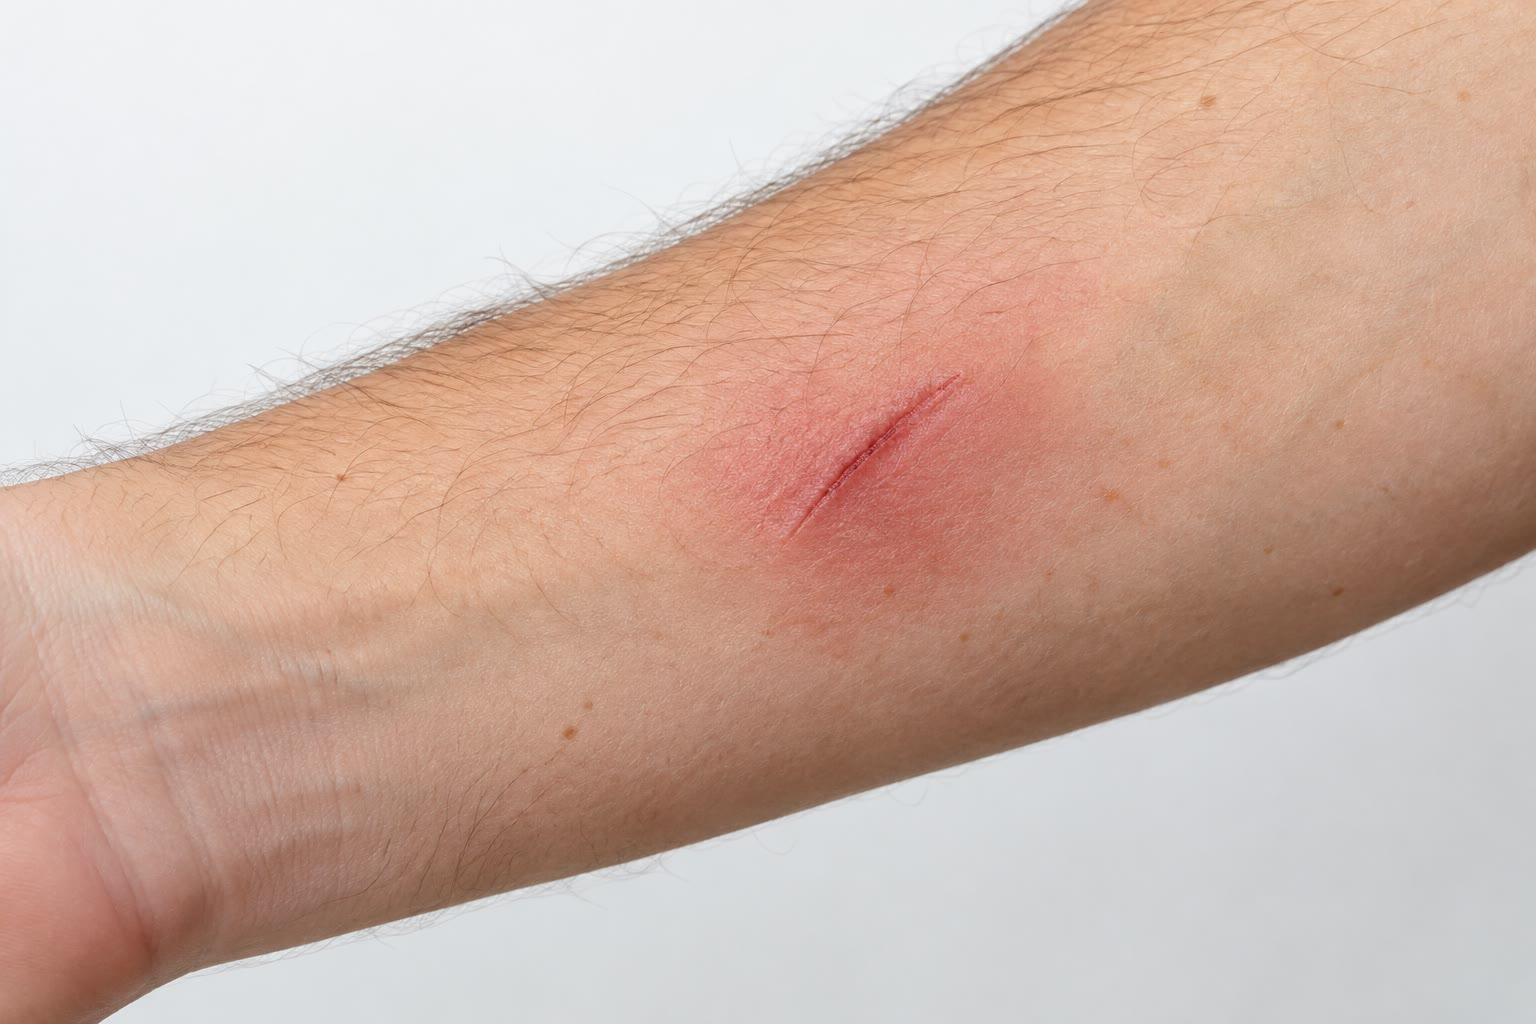
\includegraphics[width=0.52\linewidth]{images/book5/ai/b5-15-inflamed-skin.jpg}

{\small L'\omterm{def:b3:innate-immunity:inflammation}{inflammation} aiguë autour d'une griffure d'épine~: rougeur et
chaleur des vaisseaux dilatés, gonflement dû au plasma qui a fui, et la
douleur qui tient le membre immobile --- la réponse locale qui,
généralisée au corps entier, est le choc septique.}
\end{omfigure}

\section{Tuer}

\begin{definition}[La phagocytose et l'explosion oxydative]\label{def:b3:innate-immunity:killing}
\index{phagocytose}\index{explosion oxydative}\index{NADPH oxydase}\index{piège extracellulaire de neutrophile}
Un phagocyte lie sa proie par des récepteurs d'opsonines --- le C3b, et
les régions constantes des anticorps --- ou directement par des
récepteurs de motifs, l'enveloppe de membrane et referme le
\emph{phagosome}, qui fusionne avec les granules et les \omterm{def:b3:membrane-traffic:endocytosis}{lysosomes}. La
mise à mort emprunte plusieurs voies à la fois. L'\emph{explosion
oxydative}~: l'enzyme \emph{NADPH oxydase}, assemblée sur la membrane du
phagosome, pompe des électrons sur l'oxygène pour faire du superoxyde,
qui devient du peroxyde d'hydrogène, que la myéloperoxydase transforme,
avec le chlorure, en hypochlorite --- de l'eau de Javel, à concentration
millimolaire dans un compartiment d'un micromètre. Le monoxyde d'azote
de la NO synthase inductible, qui avec le superoxyde donne du
peroxynitrite. L'acide, jusqu'à pH~5. Le lysozyme, des protéases, la
lactoferrine qui affame la proie de fer, et les défensines qui la
perforent. Un \omterm{def:b3:innate-immunity:innate}{neutrophile} qui ne peut manger ce qu'il trouve --- une
hyphe fongique, un amas --- peut expulser sa propre \omterm{def:b3:chromatin-epigenetics:nucleosome}{chromatine} en un
filet collant d'ADN et de protéines de granules, un \emph{piège
extracellulaire de \omterm{def:b3:innate-immunity:innate}{neutrophile}}, et en mourir. Les enfants qui héritent
d'une NADPH oxydase défectueuse (granulomatose septique chronique)
souffrent d'abcès et de granulomes à répétition dus à des bactéries et
des champignons que les phagocytes ordinaires tuent sans peine~:
l'explosion n'est pas facultative.
\end{definition}

\begin{definition}[Les cellules tueuses naturelles et l'interféron]\label{def:b3:innate-immunity:nk-ifn}
\index{cellule tueuse naturelle!soi manquant}\index{interféron!de type I}\index{état antiviral}
Les \omterm{def:b3:virology:virus}{virus} se cachent dans les cellules, où ni le \omterm{def:b3:innate-immunity:complement}{complément} ni les
phagocytes ne peuvent les atteindre. Les \emph{\omterm{def:b3:innate-immunity:innate}{cellules tueuses
naturelles}} patrouillent à la recherche de cellules qui ont cessé
d'exposer le CMH de classe~I --- le «~soi manquant~» d'une cellule dont
l'occupant viral ou tumoral a éteint la présentation d'antigène pour
échapper aux lymphocytes~T (\cref{ch:b3:adaptive-immunity}) --- et de
protéines de stress que les cellules infectées et transformées mettent à
leur surface~; les récepteurs inhibiteurs du CMH~I et les récepteurs
activateurs des ligands de stress sont additionnés, et une cellule qui
fait pencher la balance est tuée en quelques minutes par la perforine et
les granzymes qu'on lui injecte, qui déclenchent son \omterm{def:b3:cell-cycle-apoptosis:apoptosis}{apoptose}. Les
\emph{interférons de type~I} ($\alpha$ et $\beta$) sont fabriqués par
toute cellule dont RIG-I ou cGAS a détecté un acide nucléique viral~;
sécrétés, ils se lient à des récepteurs des cellules voisines et, par la
voie JAK--STAT, induisent des centaines de gènes qui mettent ces
cellules en \emph{état \omterm{def:b3:virology:drugs}{antiviral}}~: une kinase qui arrête la traduction
quand elle rencontre de l'ARN double brin, une nucléase qui dégrade
l'ARN, des protéines qui bloquent l'entrée et l'assemblage des \omterm{def:b3:virology:virus}{virus}, et
davantage de CMH~I pour montrer aux lymphocytes~T ce qu'il y a dedans.
La cellule qui a fait l'interféron peut mourir~; ses voisines sont
prévenues. L'interféron fut découvert par Isaacs et Lindenmann (1957)
comme le facteur du milieu des cellules infectées par un \omterm{def:b3:virology:virus}{virus} qui
rendait résistantes des cellules fraîches, et c'est la raison pour
laquelle une cellule infectée par un \omterm{def:b3:virology:virus}{virus} résiste à un second.
\end{definition}

\begin{method}[Mesurer l'inflammation et la fonction phagocytaire]\label{met:b3:innate-immunity:tests}
\index{protéine C réactive!dosage}\index{test au nitrobleu de tétrazolium}
Au lit du malade~: (1) la \emph{\omterm{prop:b3:innate-immunity:systemic}{protéine C réactive}} du sérum, par
immunodosage --- au-dessous de \qty{5}{mg/L} au repos, quelques dizaines
dans une infection virale, quelques centaines dans un sepsis bactérien,
retombant en quelques jours si le traitement agit~; (2) la numération
des \omterm{def:b3:innate-immunity:innate}{neutrophiles}, élevée dans l'infection bactérienne, avec des formes
immatures relâchées tôt par la moelle~; (3) la vitesse de sédimentation
des érythrocytes, reflet lent du fibrinogène. Pour les phagocytes~: (4)
le test au \emph{nitrobleu de tétrazolium} ou à la dihydrorhodamine, où
des \omterm{def:b3:innate-immunity:innate}{neutrophiles} stimulés in vitro réduisent un colorant si leur \omterm{def:b3:innate-immunity:killing}{NADPH
oxydase} fonctionne --- le diagnostic de la granulomatose septique
chronique en une matinée~; (5) un test de chimiotactisme, qui compte les
cellules migrant à travers un filtre vers une \omterm{def:b3:innate-immunity:inflammation}{chimiokine}.
\end{method}

\section{De l'inné à l'adaptatif, et à travers le vivant}

\begin{proposition}[La décision de la cellule dendritique]\label{prop:b3:innate-immunity:bridge}
\index{cellule dendritique!maturation}\index{costimulation}\index{adjuvant}
L'immunité adaptative ne se déclenche pas toute seule. Une
\emph{\omterm{def:b3:innate-immunity:innate}{cellule dendritique}} d'un tissu mange ce qu'elle trouve~; si ses
récepteurs de motifs sont déclenchés --- par un microbe ou par un dégât
--- elle mûrit~: elle cesse de manger, migre par les lymphatiques vers
le ganglion de drainage, expose sur ses molécules de CMH les peptides de
ce qu'elle a mangé, et dresse des molécules \emph{costimulatrices} (B7)
et des \omterm{def:b3:innate-immunity:inflammation}{cytokines} qui disent à un lymphocyte~T reconnaissant le peptide
de répondre, et comment (\cref{ch:b3:adaptive-immunity}). Un
lymphocyte~T qui voit son peptide sur une \omterm{def:b3:innate-immunity:innate}{cellule dendritique} sans
costimulation est éteint. La reconnaissance innée décide donc si un
antigène mérite une réponse, et les \omterm{def:b3:innate-immunity:inflammation}{cytokines} que fait la \omterm{def:b3:innate-immunity:innate}{cellule
dendritique} --- décidées par les récepteurs de motifs qui ont tiré ---
décident si la réponse vise les \omterm{def:b3:virology:virus}{virus}, les bactéries ou les vers. Un
\emph{adjuvant} est un ligand de récepteur de motifs ajouté à un vaccin
pour fournir ce signal~; l'alun et les nanoparticules lipidiques des
vaccins modernes agissent en le déclenchant.
\end{proposition}

\begin{remark}[L'immunité innée partout, et sa mémoire]\label{rem:b3:innate-immunity:everywhere}
Tout organisme pluricellulaire possède une \omterm{def:b3:innate-immunity:innate}{immunité innée}, et les
plantes, les champignons et les invertébrés n'ont rien d'autre. Les
plantes reconnaissent la flagelline et la chitine par des récepteurs
kinases et montent une réponse à deux étages
(\cref{ch:b3:plant-molecular-physiology})~; les insectes ont Toll et des
peptides antimicrobiens~; même les bactéries ont des \omterm{def:b3:genetic-engineering:tools}{enzymes de
restriction} et \omterm{def:b3:genetic-engineering:crispr}{CRISPR} (\cref{ch:b3:genetic-engineering}). Le dogme d'une
\omterm{def:b3:innate-immunity:innate}{immunité innée} sans mémoire s'est assoupli~: un monocyte qui a rencontré
le $\beta$-glucane ou le vaccin BCG est reprogrammé épigénétiquement
(\cref{ch:b3:chromatin-epigenetics}) pour répondre plus fort à des
microbes sans rapport pendant des mois --- l'\emph{immunité entraînée},
qui explique pourquoi le BCG abaisse la mortalité infantile due à des
infections autres que la tuberculose. Et l'excès du système est une
maladie de notre temps~: l'\omterm{def:b3:innate-immunity:inflammation}{inflammation} stérile entretenue par les
cristaux d'acide urique (goutte), les cristaux de cholestérol dans la
paroi artérielle (athérosclérose), l'\omterm{def:b3:structural-biology:amyloid}{amyloïde} dans le cerveau, et
l'\omterm{def:b3:innate-immunity:inflammation}{inflammation} de bas grade de l'obésité et de la vieillesse.
\end{remark}

\section{Exercices}

\begin{exercise}[$\star$]\label{exo:b3:innate-immunity:1}
Énumérer quatre \omterm{def:b3:innate-immunity:innate}{barrières} et cinq types cellulaires de l'\omterm{def:b3:innate-immunity:innate}{immunité innée},
avec une fonction pour chacun.
\end{exercise}

\begin{exercise}[$\star$]\label{exo:b3:innate-immunity:2}
Qu'est-ce qui fait d'une molécule un bon \omterm{def:b3:innate-immunity:prr}{motif moléculaire associé aux
pathogènes}~? Donner trois exemples et le récepteur de chacun.
\end{exercise}

\begin{exercise}[$\star$]\label{exo:b3:innate-immunity:3}
Expliquer chacun des quatre signes de Celse par un médiateur et un
changement vasculaire ou nerveux.
\end{exercise}

\begin{exercise}[$\star$]\label{exo:b3:innate-immunity:4}
Nommer les trois voies du \omterm{def:b3:innate-immunity:complement}{complément}, ce qui déclenche chacune, et les
trois conséquences du clivage de C3.
\end{exercise}

\begin{exercise}[$\star\star$]\label{exo:b3:innate-immunity:5}
Dans le modèle du \omterm{def:b3:innate-immunity:complement}{complément} avec $k_{0} = 2$ par seconde, $a =
\qty{0.15}{s^{-1}}$ et $d = \qty{0.05}{s^{-1}}$ sur un microbe, combien
de C3b sont déposés après \qty{60}{s}~? Après \qty{90}{s}~? Sur une
cellule de l'hôte avec $a = 0.05$ et $d = 0.15$, quel est l'état
stationnaire~?
\end{exercise}

\begin{exercise}[$\star\star$]\label{exo:b3:innate-immunity:6}
Ordonner les événements de l'\omterm{def:b3:innate-immunity:inflammation}{extravasation}, nommer la classe de
molécules de chaque étape, et prévoir le phénotype d'un enfant dont les
\omterm{def:b3:innate-immunity:innate}{neutrophiles} manquent d'\omterm{def:b3:innate-immunity:inflammation}{intégrines} $\beta_{2}$ (déficit d'adhérence
leucocytaire).
\end{exercise}

\begin{exercise}[$\star\star$]\label{exo:b3:innate-immunity:7}
Les \omterm{def:b3:innate-immunity:innate}{neutrophiles} d'un patient échouent au test à la dihydrorhodamine.
Quel est le diagnostic, quelle réaction manque, et à quelles infections
s'attendre~? Pourquoi des granulomes se forment-ils~?
\end{exercise}

\begin{exercise}[$\star\star$]\label{exo:b3:innate-immunity:8}
Expliquer la reconnaissance du soi manquant et prévoir ce qu'il advient
d'une cellule tumorale qui (a) perd le CMH~I pour échapper aux
lymphocytes~T, (b) garde le CMH~I mais expose des ligands de stress.
\end{exercise}

\begin{exercise}[$\star\star$]\label{exo:b3:innate-immunity:9}
Pourquoi un vaccin de protéine pure induit-il peu d'immunité, et
qu'ajoute un adjuvant~? Relier à l'argument de Janeway.
\end{exercise}

\begin{exercise}[$\star\star\star$]\label{exo:b3:innate-immunity:10}
La fièvre coûte \qty{12}{\%} du métabolisme de repos par degré et
allonge le temps de doublement d'une bactérie de \qty{30}{min} à
\qty{37}{\celsius} à \qty{45}{min} à \qty{40}{\celsius}. Sur un jour
d'infection, calculer la population bactérienne à partir de $10^{4}$
avec et sans fièvre (en négligeant la destruction), et l'énergie
supplémentaire pour une personne à \qty{8}{MJ/d}. La fièvre en vaut-elle
la peine~? De quoi la réponse dépend-elle~?
\end{exercise}

\begin{exercise}[$\star\star\star$]\label{exo:b3:innate-immunity:11}
Certaines bactéries fixent le facteur H à leur surface~; d'autres
clivent le C3b ou perdent leur capsule. À l'aide du
\cref{thm:b3:innate-immunity:complement}, expliquer chacune comme un
changement de $a$ ou de $d$, et dire laquelle est la défense la plus
économique pour le microbe.
\end{exercise}

\begin{exercise}[$\star\star\star$]\label{exo:b3:innate-immunity:12}
Argumenter, avec les mécanismes de ce chapitre, pourquoi la même réponse
est adaptative au niveau d'une écharde et létale dans la circulation
sanguine, et pourquoi les médicaments qui bloquent le TNF aident dans la
polyarthrite rhumatoïde mais augmentent le risque de tuberculose.
\end{exercise}

\section{Problème~: une écharde}

\begin{problem}[{Problème du week-end --- dix mille bactéries sous la
peau lancées dans une course contre les neutrophiles envoyés à leur
rencontre, couvertes de complément par l'arithmétique de la boucle,
combattues par la fièvre à son prix métabolique et, dans le sang,
transformées en physiologie du choc, pour finir sur les bactéries
restantes après six heures, le C3b sur chacune et le coût d'une journée
de fièvre}]
\label{pb:b3:innate-immunity:1}
Données~: $10^{4}$ bactéries inoculées, doublant toutes les
\qty{40}{min}~; les \omterm{def:b3:innate-immunity:innate}{neutrophiles} arrivent à partir de \qty{1}{h} au
rythme de $2\times 10^{4}$ par heure, chacun tuant $20$ bactéries puis
mourant. \omterm{def:b3:innate-immunity:complement}{Complément}~: $k_{0} = 1$ par seconde et par bactérie,
$a - d = \qty{0.08}{s^{-1}}$ sur les bactéries, $d - a =
\qty{0.1}{s^{-1}}$ sur les cellules de l'hôte~; la surface d'une
bactérie ne porte au plus que $2\times 10^{6}$ C3b. Fièvre~:
$+\qty{2}{\celsius}$ coûte \qty{24}{\%} d'un métabolisme de
\qty{8}{MJ/d} et allonge le temps de doublement bactérien à
\qty{60}{min}. Sepsis~: $10^{9}$ bactéries dans \qty{5}{L} de sang,
$3\times 10^{6}$ molécules de \omterm{def:b3:bacteriology:envelope}{lipopolysaccharide} par bactérie~; la
signalisation TLR4 sature à $10^{-9}$ mol/L de \omterm{def:b3:bacteriology:envelope}{lipopolysaccharide}.

\medskip
\noindent\textbf{Partie I --- La course.}
\begin{enumerate}
  \item Combien de bactéries à \qty{1}{h}, quand arrivent les premiers
        \omterm{def:b3:innate-immunity:innate}{neutrophiles}, si aucune n'a été tuée~?
  \item Entre \qty{1}{h} et \qty{2}{h}, combien de \omterm{def:b3:innate-immunity:innate}{neutrophiles} arrivent
        et combien de bactéries peuvent-ils tuer~? Comparer à la
        croissance bactérienne de cette heure-là à partir du compte de
        la question 1.
  \item Continuer heure par heure (croissance, puis destruction à la fin
        de chaque heure) jusqu'à \qty{6}{h}. Quand la population
        culmine-t-elle, et combien en reste-t-il à \qty{6}{h}~?
  \item Refaire avec une arrivée des \omterm{def:b3:innate-immunity:innate}{neutrophiles} retardée à \qty{3}{h}.
        Que se passe-t-il à \qty{6}{h}~? Commenter la valeur de la
        rapidité.
  \item Combien de \omterm{def:b3:innate-immunity:innate}{neutrophiles} morts se sont accumulés quand les
        bactéries ont disparu à la question 3~? Qu'est-ce que le pus, et
        pourquoi doit-il être évacué~?
  \item Une personne ayant le dixième du compte normal de \omterm{def:b3:innate-immunity:innate}{neutrophiles}
        (neutropénie après chimiothérapie)~: refaire la question 3 et
        expliquer pourquoi de tels patients reçoivent des \omterm{def:b3:bacteriology:antibiotics}{antibiotiques}
        dès la première fièvre.
\end{enumerate}

\medskip
\noindent\textbf{Partie II --- Le manteau.}
\begin{enumerate}[resume]
  \item D'après le théorème, combien de C3b sont déposés sur une
        bactérie après \qty{30}{s}, \qty{60}{s} et \qty{120}{s}~?
  \item Quand la surface sature-t-elle~?
  \item Sur une cellule de l'hôte à côté, quel est le nombre
        stationnaire de C3b~?
  \item La bactérie acquiert une capsule qui divise $a$ par deux, de
        sorte que $a -
        d = 0.03$. Recalculer le C3b à \qty{120}{s}. Qu'achète la
        capsule~?
  \item Combien de C3b l'inoculum entier de $10^{4}$ bactéries
        porte-t-il à saturation, et quelle fraction cela fait-il des
        $2\times 10^{16}$ molécules de C3 d'un litre de plasma~?
  \item Un patient manque de C3. Quelles voies sont touchées, et quelles
        infections s'ensuivent~? Un patient manque de C9~: pourquoi le
        phénotype est-il plus modéré, et limité à un seul genre~?
\end{enumerate}

\medskip
\noindent\textbf{Partie III --- La fièvre.}
\begin{enumerate}[resume]
  \item Combien d'énergie supplémentaire coûtent deux jours de fièvre à
        $+\qty{2}{\celsius}$, en mégajoules et en grammes de graisse
        (\qty{38}{kJ/g})~?
  \item Refaire la question 1 à la température de fièvre~: combien de
        bactéries à \qty{1}{h}~? De quel facteur la fièvre a-t-elle
        réduit la population que rencontrent les \omterm{def:b3:innate-immunity:innate}{neutrophiles}~?
  \item Dans le modèle de la question 3, avec le temps de doublement
        allongé, quand les bactéries ont-elles disparu~?
  \item La \omterm{prop:b3:innate-immunity:systemic}{protéine C réactive} passe de \qty{1}{mg/L} à \qty{200}{mg/L}
        en deux jours. Avec un volume plasmatique de \qty{3}{L} et une
        masse moléculaire de \qty{115}{kDa}, combien de molécules le
        foie a-t-il fabriquées, et combien par seconde~?
  \item Les antipyrétiques bloquent la synthèse des prostaglandines. Que
        font-ils à la consigne, au confort du patient et, d'après les
        nombres ci-dessus, à l'infection~?
  \item Pourquoi une fièvre à \qty{41}{\celsius} est-elle dangereuse
        quand \qty{39}{\celsius} ne l'est pas, et qu'est-ce qui empêche
        la consigne de monter indéfiniment~?
\end{enumerate}

\medskip
\noindent\textbf{Partie IV --- Le choc.}
\begin{enumerate}[resume]
  \item Les molécules de \omterm{def:b3:bacteriology:envelope}{lipopolysaccharide} dans le sang du patient
        septique, et leur concentration en mol/L.
  \item Comparer à la concentration saturante pour TLR4. Les \omterm{def:b3:innate-immunity:innate}{macrophages}
        du corps sont-ils tous activés~?
  \item Chacun des $10^{11}$ \omterm{def:b3:innate-immunity:innate}{macrophages} du corps libère \num{1000}
        molécules de TNF par seconde pendant une heure. Combien de moles
        de TNF, et quelle concentration dans \qty{15}{L} de liquide
        extracellulaire~? (Le TNF agit à \qty{1e-11}{mol/L}.)
  \item Expliquer la chute de la pression artérielle et la défaillance
        des reins à partir des mécanismes locaux de l'\omterm{def:b3:innate-immunity:inflammation}{inflammation}.
  \item L'\omterm{def:b3:bacteriology:antibiotics}{antibiotique} donné à l'admission tue les bactéries en une
        heure. Pourquoi le patient peut-il s'aggraver avant de
        s'améliorer, et qu'est-ce qui limite l'utilité des anticorps
        anti-TNF dans le sepsis~?
  \item Une souche de souris manque de TLR4. Prévoir sa réponse au
        \omterm{def:b3:bacteriology:envelope}{lipopolysaccharide} injecté et à une infection vivante à \omterm{def:b3:bacteriology:envelope}{Gram
        négatif}, et expliquer le paradoxe apparent.
  \item Résumer~: les bactéries restantes à \qty{6}{h} (question~3), le
        C3b sur une bactérie à \qty{120}{s} (question~7), et le coût de
        deux jours de fièvre (question~13).
\end{enumerate}
\end{problem}
